\documentclass{extarticle}
\usepackage[a4paper, total={6.5in, 9.2in}]{geometry}
\usepackage[T1]{fontenc}
\usepackage{times}
\usepackage{verbatim}
\usepackage{graphicx}
\usepackage{amsmath}


\title{Sampling non-isotropic Gaussian random fields}
\author{}
\date{}
\begin{document}
\maketitle
\texttt{RandField\_Matern.m} script  uses the following stationary non-isotropic Mat\'ern model 
\begin{align}
C_\Phi(\mathbf{x_1},\mathbf{x_2}) &= \sigma_c^2\dfrac{2^{1-\nu_c}}{\Gamma(\nu_c)}\left( 2\sqrt{\nu_c}\tilde{r}\right)^{\nu_c} K_{\nu_c}\left( 2\sqrt{\nu_c}\tilde{r}\right)\\
\tilde{r}  &= \sqrt{\dfrac{(x_1-x_2)^2}{\lambda^2_{cx}}+ \dfrac{(y_1-y_2)^2}{\lambda^2_{cy}}}\quad\text{with}\quad \mathbf{x_1} = (x_1,y_1),\mathbf{x_2} = (x_2,y_2).
\end{align}
where $\lambda_{cx}$ and $\lambda_{cy}$ are correlation lengths along x- and y-coordinates, respectively, $\nu_c$ is the smoothness of the random field and $\sigma^2_c$ is the marginal variance. Some examples of usage:

\vspace{1cm}
\texttt{>>[F]= RandField\_Matern(0.1,0.1,1,1,7,1)\% isotropic}\\
\centering
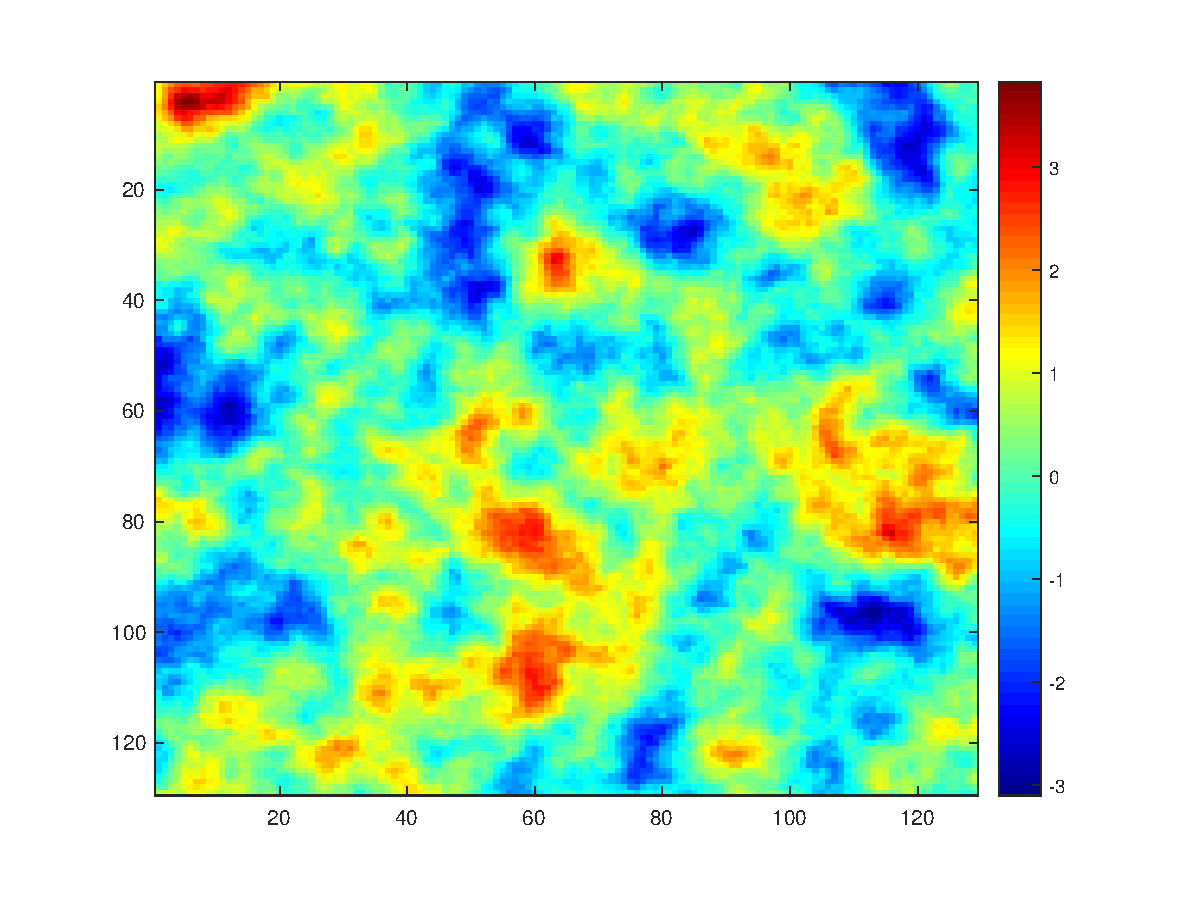
\includegraphics[scale=0.4]{f1.eps}\\
\texttt{>>[F]= RandField\_Matern(2,0.02,0.5,1,7,1)\% layering along x}\\
\centering
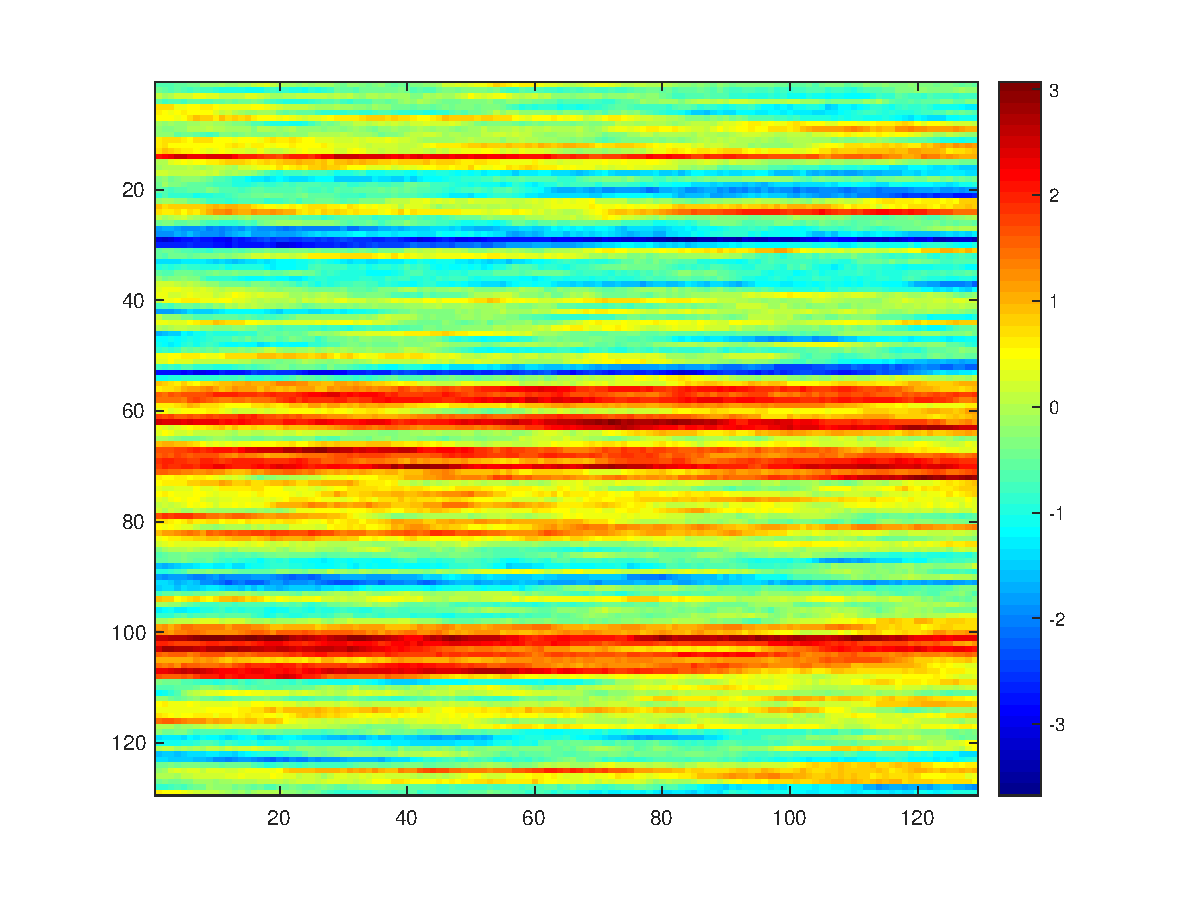
\includegraphics[scale=0.4]{f2.eps}\\
\texttt{>>[F]= RandField\_Matern(0.01,1,0.5,0.5,7,1) \% layering along y}\\
\centering
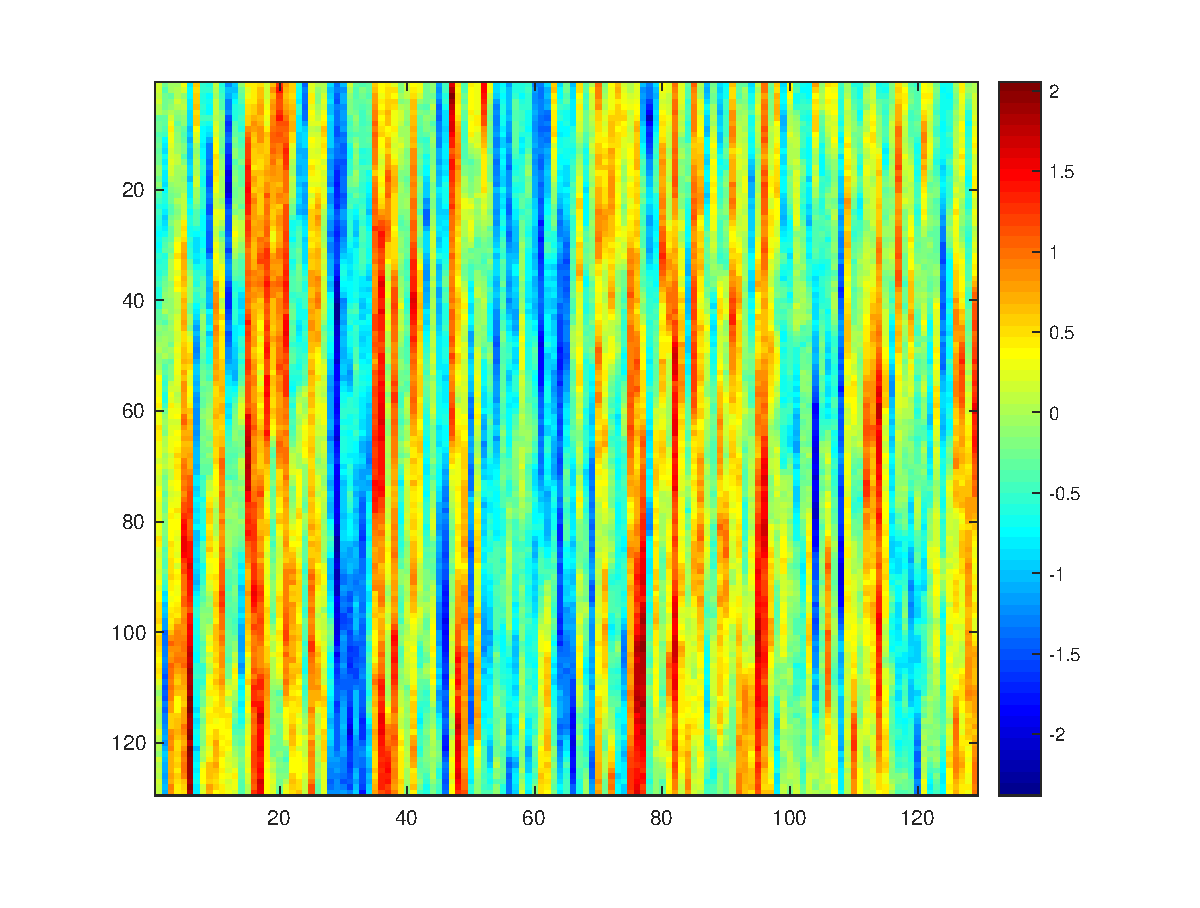
\includegraphics[scale=0.4]{f3.eps}


\end{document}